% Options for packages loaded elsewhere
\PassOptionsToPackage{unicode}{hyperref}
\PassOptionsToPackage{hyphens}{url}
%
\documentclass[
]{article}
\usepackage{amsmath,amssymb}
\usepackage{iftex}
\ifPDFTeX
  \usepackage[T1]{fontenc}
  \usepackage[utf8]{inputenc}
  \usepackage{textcomp} % provide euro and other symbols
\else % if luatex or xetex
  \usepackage{unicode-math} % this also loads fontspec
  \defaultfontfeatures{Scale=MatchLowercase}
  \defaultfontfeatures[\rmfamily]{Ligatures=TeX,Scale=1}
\fi
\usepackage{lmodern}
\ifPDFTeX\else
  % xetex/luatex font selection
\fi
% Use upquote if available, for straight quotes in verbatim environments
\IfFileExists{upquote.sty}{\usepackage{upquote}}{}
\IfFileExists{microtype.sty}{% use microtype if available
  \usepackage[]{microtype}
  \UseMicrotypeSet[protrusion]{basicmath} % disable protrusion for tt fonts
}{}
\makeatletter
\@ifundefined{KOMAClassName}{% if non-KOMA class
  \IfFileExists{parskip.sty}{%
    \usepackage{parskip}
  }{% else
    \setlength{\parindent}{0pt}
    \setlength{\parskip}{6pt plus 2pt minus 1pt}}
}{% if KOMA class
  \KOMAoptions{parskip=half}}
\makeatother
\usepackage{xcolor}
\usepackage[margin=1in]{geometry}
\usepackage{color}
\usepackage{fancyvrb}
\newcommand{\VerbBar}{|}
\newcommand{\VERB}{\Verb[commandchars=\\\{\}]}
\DefineVerbatimEnvironment{Highlighting}{Verbatim}{commandchars=\\\{\}}
% Add ',fontsize=\small' for more characters per line
\usepackage{framed}
\definecolor{shadecolor}{RGB}{248,248,248}
\newenvironment{Shaded}{\begin{snugshade}}{\end{snugshade}}
\newcommand{\AlertTok}[1]{\textcolor[rgb]{0.94,0.16,0.16}{#1}}
\newcommand{\AnnotationTok}[1]{\textcolor[rgb]{0.56,0.35,0.01}{\textbf{\textit{#1}}}}
\newcommand{\AttributeTok}[1]{\textcolor[rgb]{0.13,0.29,0.53}{#1}}
\newcommand{\BaseNTok}[1]{\textcolor[rgb]{0.00,0.00,0.81}{#1}}
\newcommand{\BuiltInTok}[1]{#1}
\newcommand{\CharTok}[1]{\textcolor[rgb]{0.31,0.60,0.02}{#1}}
\newcommand{\CommentTok}[1]{\textcolor[rgb]{0.56,0.35,0.01}{\textit{#1}}}
\newcommand{\CommentVarTok}[1]{\textcolor[rgb]{0.56,0.35,0.01}{\textbf{\textit{#1}}}}
\newcommand{\ConstantTok}[1]{\textcolor[rgb]{0.56,0.35,0.01}{#1}}
\newcommand{\ControlFlowTok}[1]{\textcolor[rgb]{0.13,0.29,0.53}{\textbf{#1}}}
\newcommand{\DataTypeTok}[1]{\textcolor[rgb]{0.13,0.29,0.53}{#1}}
\newcommand{\DecValTok}[1]{\textcolor[rgb]{0.00,0.00,0.81}{#1}}
\newcommand{\DocumentationTok}[1]{\textcolor[rgb]{0.56,0.35,0.01}{\textbf{\textit{#1}}}}
\newcommand{\ErrorTok}[1]{\textcolor[rgb]{0.64,0.00,0.00}{\textbf{#1}}}
\newcommand{\ExtensionTok}[1]{#1}
\newcommand{\FloatTok}[1]{\textcolor[rgb]{0.00,0.00,0.81}{#1}}
\newcommand{\FunctionTok}[1]{\textcolor[rgb]{0.13,0.29,0.53}{\textbf{#1}}}
\newcommand{\ImportTok}[1]{#1}
\newcommand{\InformationTok}[1]{\textcolor[rgb]{0.56,0.35,0.01}{\textbf{\textit{#1}}}}
\newcommand{\KeywordTok}[1]{\textcolor[rgb]{0.13,0.29,0.53}{\textbf{#1}}}
\newcommand{\NormalTok}[1]{#1}
\newcommand{\OperatorTok}[1]{\textcolor[rgb]{0.81,0.36,0.00}{\textbf{#1}}}
\newcommand{\OtherTok}[1]{\textcolor[rgb]{0.56,0.35,0.01}{#1}}
\newcommand{\PreprocessorTok}[1]{\textcolor[rgb]{0.56,0.35,0.01}{\textit{#1}}}
\newcommand{\RegionMarkerTok}[1]{#1}
\newcommand{\SpecialCharTok}[1]{\textcolor[rgb]{0.81,0.36,0.00}{\textbf{#1}}}
\newcommand{\SpecialStringTok}[1]{\textcolor[rgb]{0.31,0.60,0.02}{#1}}
\newcommand{\StringTok}[1]{\textcolor[rgb]{0.31,0.60,0.02}{#1}}
\newcommand{\VariableTok}[1]{\textcolor[rgb]{0.00,0.00,0.00}{#1}}
\newcommand{\VerbatimStringTok}[1]{\textcolor[rgb]{0.31,0.60,0.02}{#1}}
\newcommand{\WarningTok}[1]{\textcolor[rgb]{0.56,0.35,0.01}{\textbf{\textit{#1}}}}
\usepackage{longtable,booktabs,array}
\usepackage{calc} % for calculating minipage widths
% Correct order of tables after \paragraph or \subparagraph
\usepackage{etoolbox}
\makeatletter
\patchcmd\longtable{\par}{\if@noskipsec\mbox{}\fi\par}{}{}
\makeatother
% Allow footnotes in longtable head/foot
\IfFileExists{footnotehyper.sty}{\usepackage{footnotehyper}}{\usepackage{footnote}}
\makesavenoteenv{longtable}
\usepackage{graphicx}
\makeatletter
\def\maxwidth{\ifdim\Gin@nat@width>\linewidth\linewidth\else\Gin@nat@width\fi}
\def\maxheight{\ifdim\Gin@nat@height>\textheight\textheight\else\Gin@nat@height\fi}
\makeatother
% Scale images if necessary, so that they will not overflow the page
% margins by default, and it is still possible to overwrite the defaults
% using explicit options in \includegraphics[width, height, ...]{}
\setkeys{Gin}{width=\maxwidth,height=\maxheight,keepaspectratio}
% Set default figure placement to htbp
\makeatletter
\def\fps@figure{htbp}
\makeatother
\setlength{\emergencystretch}{3em} % prevent overfull lines
\providecommand{\tightlist}{%
  \setlength{\itemsep}{0pt}\setlength{\parskip}{0pt}}
\setcounter{secnumdepth}{-\maxdimen} % remove section numbering
\ifLuaTeX
  \usepackage{selnolig}  % disable illegal ligatures
\fi
\IfFileExists{bookmark.sty}{\usepackage{bookmark}}{\usepackage{hyperref}}
\IfFileExists{xurl.sty}{\usepackage{xurl}}{} % add URL line breaks if available
\urlstyle{same}
\hypersetup{
  pdftitle={Modèles d'équations structuraux},
  hidelinks,
  pdfcreator={LaTeX via pandoc}}

\title{Modèles d'équations structuraux}
\author{}
\date{\vspace{-2.5em}}

\begin{document}
\maketitle

{
\setcounter{tocdepth}{2}
\tableofcontents
}
\hypertarget{introduction}{%
\section{Introduction}\label{introduction}}

Les modèles d'équations structurelles appartiennent à une famille de
modèles qui consistent en un ensemble d'équations mathématiques et
d'hypothèses sur un système étudié. Ces hypothèses découlent de nos
connaissances préalables ou de nos suppositions sur le fonctionnement du
système. En statistique, un système est un ensemble de variables ou de
phénomènes qui sont étudiés dans le cadre d'une analyse ou d'une étude.
Ces variables peuvent être liées par des relations complexes. Notre
objectif avec l'analyse est de comprendre comment ces variables
interagissent les unes avec les autres ou comment elles influencent un
résultat ou un phénomène en particulier.

\hypertarget{contenu-du-cours}{%
\section{Contenu du cours}\label{contenu-du-cours}}

\begin{itemize}
\item
  Types de variables et relations dans un modèle d'équations
  structurelles ;
\item
  Du modèle théorique au modèle statistique ;
\item
  Ajustement du modèle dans lavaan.
\end{itemize}

\hypertarget{types-des-variables-et-liens-dans-un-moduxe8le-duxe9quation-structurel}{%
\section{Types des variables et liens dans un modèle d'équation
structurel:}\label{types-des-variables-et-liens-dans-un-moduxe8le-duxe9quation-structurel}}

La structure théorique d'un modèle d'équations structurelles englobe
plusieurs types de variables, définissant leurs caractéristiques et
leurs rôles dans le modèle.

Selon leur \textbf{nature}, les variables peuvent être classées en 1)
\textbf{variables latentes} et 2) \textbf{variables observées}. Une
\textbf{variable latente} est une variable qui n'est pas mesurée
directement, mais qui représente des concepts ou des traits qui n'ont
pas vraiment d'unité de mesure. Il s'agit d'un type de variable plus
souvent utilisé en psychologie (l'intelligence, la satisfaction, etc.).
Les \textbf{variables observées} sont des variables mesurées ou
collectées avec des méthodes établies par la discipline. En écologie,
nous travaillons souvent avec des variables observées.

Selon le \textbf{rôle} des variables dans le modèle théorique, les
variables peuvent être \textbf{exogènes} ou \textbf{endogènes}. Les
\textbf{variables exogènes} sont des variables indépendantes qui
influencent les autres variables dans les modèles, mais qui ne sont pas
influencées par aucune autre variable en retour. Elles représentent les
moteurs des changements dans notre système. Les \textbf{variables
endogènes}, vice-versa, sont des variables qui sont influencées par les
variables exogènes ou d'autres variables du modèle, et représentent
normalement le noyau de notre système et les résultats des processus que
nous sommes en train de décrire avec notre modèle.

Selon la façon dont les variables sont conceptualisées dans le modèles,
les variables peuvent avoir un statut de modérateur et de médiateur. Un
\textbf{modérateur} est une variable qui influence la force et la
direction du lien entre deux variables. Une variable modératrice
n'explique pas les ``causes'' du lien, mais elle intervient seulement
dans les aspects quantitatives de la relation étudiée entre deux
variables. Un \textbf{médiateur} est une variable qui explique le lien
entre une variable indépendante et une variable dépendante. Une variable
agit comme variable médiatrice lorsque elle représente la cause du lien
entre deux variables.

\begin{figure}
\centering
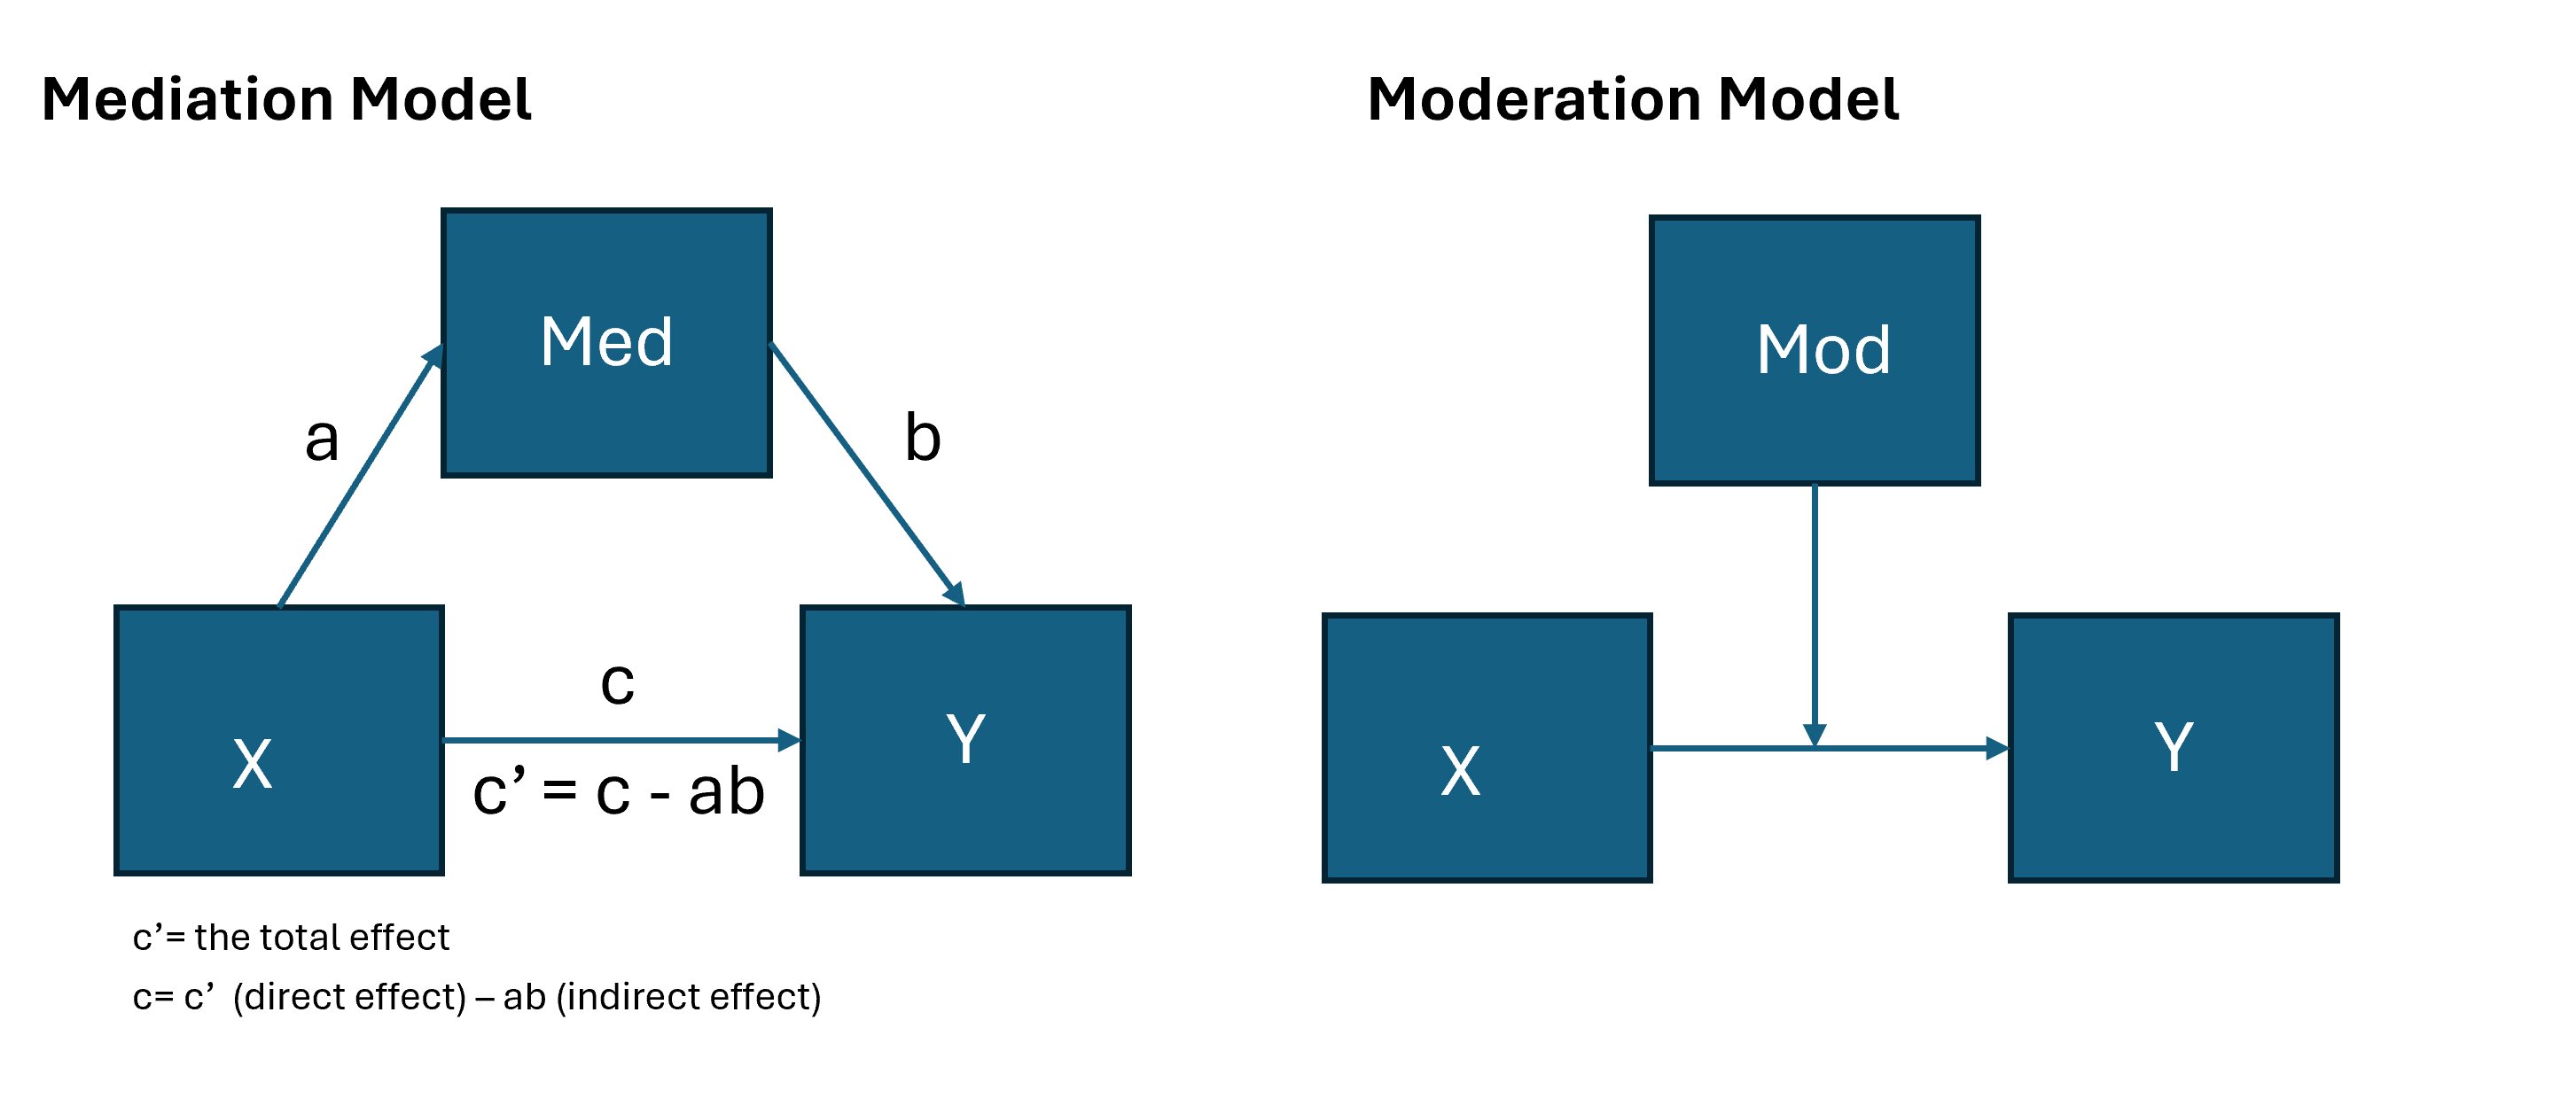
\includegraphics{C:/Users/buttoval/Documents/ECL8202/notes_cours/modmed.png}
\caption{Modèles pour une analyses de Médiation et une analyses des
moderateurs}
\end{figure}

Dans la figure, les fléchés représentent des \textbf{chemin}. Dans un
modèle d'équations structurelles un chémin répresnete une relation qui
relie deux variables, pouvant être directe ou indirecte, et pouvant
inclure des effets médiatisés. Comme vous pouvez le voir dans l'image,
les effets médiatisés se réfèrent à une situation où l'impact d'une
variable indépendante sur une variable dépendante passe par une autre
variable. Autrement dit, la variable médiatrice transmet ou médie
l'effet de la variable indépendante sur la variable dépendante.

Dans un modèle d'équations structurelles, l'analyse de médiation et e
modération sont intégrées pour obtenir une compréhension plus profonde
des relations entre nos variables, en tenant compte à la fois de
processus médiatiques et des effets des modérateurs. Cependant, on peut
réaliser des analyses des modérateurs et de médiateurs si on souhaite
tester des les relations entres trois variables avec le package Psych:

La fonction `mediate' du package `psych' vous permet de conduire une
analyse de médiation avec la fonction `mediate'. La variable médiatrice
doit être mise entre parenthèses afin d'informer la fonction de son rôle
dans le modèle. Dans l'exemple que nous allons utiliser pour montrer la
fonction, nous utilisons la fonction `mediate' pour tester les effets
directs et indirects de la température sur la largeur des cernes de
croissance. En effet, dans l'hémisphère nord et dans des environnements
froids où la température est un facteur limitant pour la croissance, la
largeur des cernes de croissance augmente avec la température.
Cependant, la largeur du cerne de croissance est étroitement liée au
nombre de cellules du bois qui composent le cerne, et qui est, à son
tour, reliée à la température. Ainsi, une partie de l'effet total de la
température sur la largeur du cerne est en effet médiée par le nombre de
cellules. Si l'effet direct de la température sur le nombre de cellules
est plus grand par rapport à celui sur la largeur du cerne, les
changements de température seront plus liés aux changements du nombre de
cellules qu'à la largeur du cerne, et donc ces derniers seront plus
facilement prédictibles.

\begin{Shaded}
\begin{Highlighting}[]
\FunctionTok{require}\NormalTok{(psych)}
\end{Highlighting}
\end{Shaded}

\begin{verbatim}
## Le chargement a nécessité le package : psych
\end{verbatim}

\begin{verbatim}
## Warning: le package 'psych' a été compilé avec la version R 4.3.3
\end{verbatim}

\begin{Shaded}
\begin{Highlighting}[]
\NormalTok{ringdatacell }\OtherTok{\textless{}{-}} \FunctionTok{read.csv}\NormalTok{(}\StringTok{"C:/Users/buttoval/Documents/ECL8202/donnees//ringdatacell.CSV"}\NormalTok{)}


\NormalTok{medanalysys}\OtherTok{\textless{}{-}}\FunctionTok{mediate}\NormalTok{( ring\_width }\SpecialCharTok{\textasciitilde{}}\NormalTok{ temperature }\SpecialCharTok{+}\NormalTok{ (cell\_number) , }\AttributeTok{data=}\NormalTok{ringdatacell )}
\end{Highlighting}
\end{Shaded}

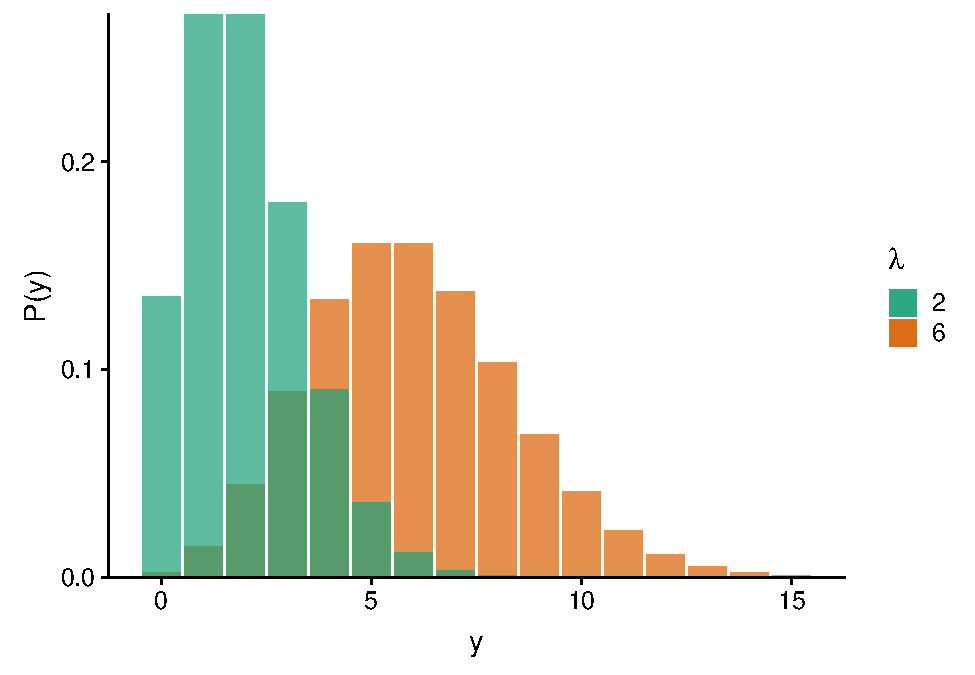
\includegraphics{08-new-SEM_files/figure-latex/unnamed-chunk-1-1.pdf}

Dans le schéma on voit très bien que l'effet totale de la température
est c = 8.15, mais l'effet direct de la temperature sur le cerne de
croissance c'= 0.56, est beaucoup plus petit.

\emph{Nota bene} la fonction ``mediate'' nous donne les coefficients
standardisées par defaut, ainsi que les moyennes centrées. pour éviter
cela il faut utiliser les aurgments ``zero=FALSE'' et std=FALSE.

\begin{Shaded}
\begin{Highlighting}[]
\FunctionTok{summary}\NormalTok{(medanalysys)}
\end{Highlighting}
\end{Shaded}

\begin{verbatim}
## Call: mediate(y = ring_width ~ temperature + (cell_number), data = ringdatacell)
## 
## Direct effect estimates (traditional regression)    (c') X + M on Y 
##             ring_width     se     t df     Prob
## Intercept      -157.63 459.43 -0.34 97 7.32e-01
## temperature     293.58  44.61  6.58 97 2.38e-09
## cell_number       8.18  21.29  0.38 97 7.02e-01
## 
## R = 0.84 R2 = 0.7   F = 112.67 on 2 and 97 DF   p-value:  5.08e-26 
## 
##  Total effect estimates (c) (X on Y) 
##             ring_width     se     t df     Prob
## Intercept       -93.82 426.50 -0.22 98 8.26e-01
## temperature     308.78  20.49 15.07 98 2.88e-27
## 
##  'a'  effect estimates (X on M) 
##             cell_number   se     t df     Prob
## Intercept          7.80 2.03  3.84 98 2.20e-04
## temperature        1.86 0.10 19.04 98 1.06e-34
## 
##  'b'  effect estimates (M on Y controlling for X) 
##             ring_width    se    t df  Prob
## cell_number       8.18 21.29 0.38 97 0.702
## 
##  'ab'  effect estimates (through all  mediators)
##             ring_width  boot    sd  lower upper
## temperature      15.21 14.17 43.48 -70.94  99.2
\end{verbatim}

Dans une analyse de modération, on examine comment l'effet d'une
variable indépendante sur une variable dépendante peut être modifié par
une autre variable, appelée modérateur. Pour évaluer cette interaction,
on inclut généralement un terme d'interaction dans le modèle de
régression multiple. Ce terme d'interaction permet de tester si l'effet
de la variable indépendante sur la variable dépendante varie en fonction
des niveaux du modérateur. En résumé, une analyse de modération est une
régression multiple avec une interaction. On peut obtenir un modèle de
modération en utilisant la fonction médiate, mais sans spécifier l'effet
du modérateur.

\begin{Shaded}
\begin{Highlighting}[]
\NormalTok{medanalysys}\OtherTok{\textless{}{-}}\FunctionTok{mediate}\NormalTok{( ring\_width }\SpecialCharTok{\textasciitilde{}}\NormalTok{   cell\_number  }\SpecialCharTok{+}\NormalTok{ moisture }\SpecialCharTok{+}\NormalTok{ moisture}\SpecialCharTok{*}\NormalTok{temperature, }
                      \AttributeTok{data=}\NormalTok{ringdatacell,}\AttributeTok{zero=} \ConstantTok{FALSE}\NormalTok{,}\AttributeTok{std=}\ConstantTok{FALSE}\NormalTok{)}
\end{Highlighting}
\end{Shaded}

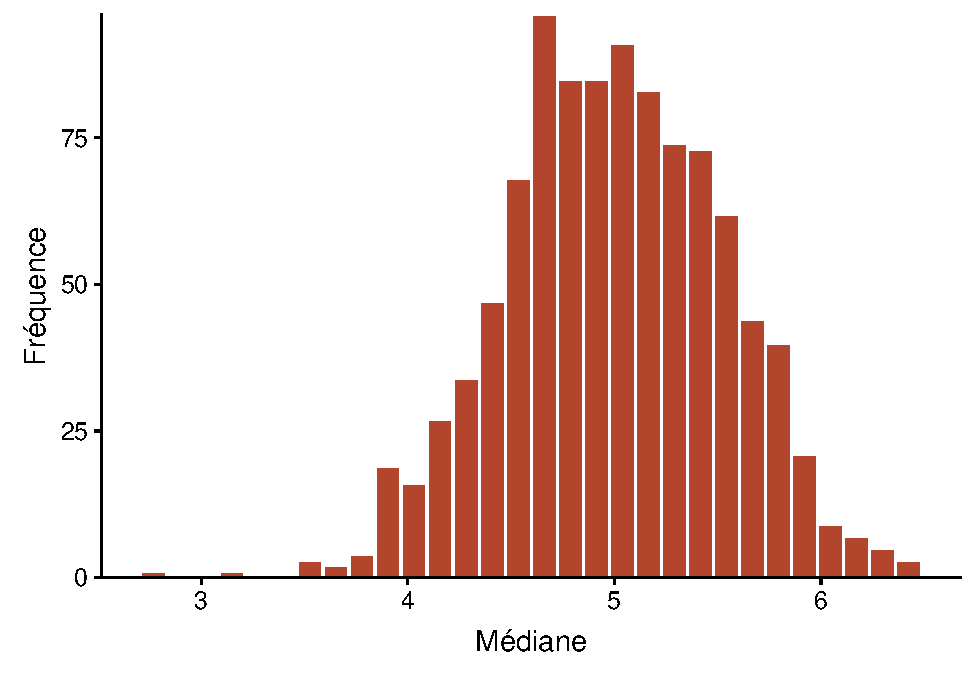
\includegraphics{08-new-SEM_files/figure-latex/unnamed-chunk-3-1.pdf}

\begin{Shaded}
\begin{Highlighting}[]
\FunctionTok{summary}\NormalTok{(medanalysys)}
\end{Highlighting}
\end{Shaded}

\begin{verbatim}
## Call: mediate(y = ring_width ~ cell_number + moisture + moisture * 
##     temperature, data = ringdatacell, std = FALSE, zero = FALSE)
## 
## No mediator specified leads to traditional regression 
##                      ring_width    se      t df      Prob
## Intercept                  9.04 11.16   0.81 95  4.20e-01
## cell_number                3.45  0.13  27.50 95  4.97e-47
## moisture                  -0.08  0.22  -0.33 95  7.39e-01
## temperature                1.02  0.66   1.55 95  1.25e-01
## moisture*temperature       6.00  0.01 522.12 95 4.55e-166
## 
## R = 1 R2 = 1   F = 2400995 on 4 and 95 DF   p-value:  9.14e-237
\end{verbatim}

\hypertarget{du-moduxe8le-thuxe9orique-au-moduxe8le-statistique}{%
\subsection{Du modèle théorique au modèle
statistique:}\label{du-moduxe8le-thuxe9orique-au-moduxe8le-statistique}}

Lorsqu'on décide de réaliser une SEM, une hypothèse bien définie
représente le meilleur investissement pour valoriser cette analyse. Nous
allons donc classer nos variables selon la typologie définie dans le
paragraphe précédent, puis construire notre modèle \textbf{a priori}. Ce
modèle représente notre compréhension du système basée sur les preuves
scientifiques que nous avons recueillies dans notre étude, et contient
nos hypothèses sous forme de liens entre les variables.

Dans une SEM, on établit un modèle théorique basé sur des relations
postulées entre les variables, puis on teste ce modèle avec des données
réelles pour voir s'il correspond bien à ces données. L'objectif est de
déterminer si le modèle théorique est statistiquement valide et peut
être généralisé aux données réelles. La validation du modèle nécessite
donc de ne pas rejeter l'hypothèse nulle selon laquelle les relations
entre les variables telles qu'elles sont spécifiées dans le modèle
théorique sont également présentes dans les données réelles, et que
toute différence observée entre le modèle théorique et les données
réelles est due au hasard ou à des erreurs de mesures.

Dans un SEM, on peut utilier des symboles peuvent être utilisés pour
représenter les liens et les variables dansun diagramme:

\begin{figure}
\centering
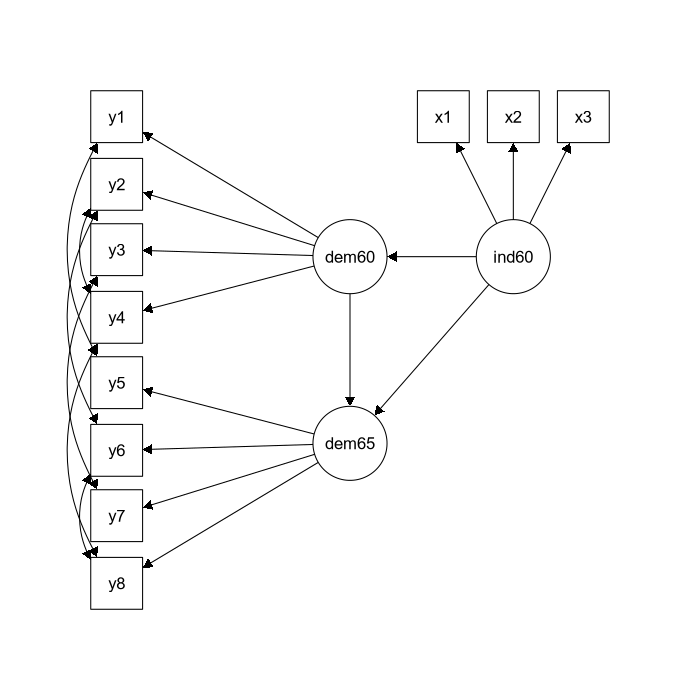
\includegraphics{C:/Users/buttoval/Documents/ECL8202/notes_cours/sem.png}
\caption{Symboles pour les diagrammes}
\end{figure}

Il y a plusieurs packages qui peuvent vous permettre de réaliser un
modèle SEM sur R. Ici nous allons utiliser Lavaan, qui utilise ça propre
syntaxe pour définir les variables du modèle et leur liens.

\begin{longtable}[]{@{}lll@{}}
\toprule\noalign{}
Formule et définition & operateur & signification \\
\midrule\noalign{}
\endhead
\bottomrule\noalign{}
\endlastfoot
variable latente & =\textasciitilde{} & obtenue à partir de \\
Covariable & \textasciitilde\textasciitilde{} & est correlé avec \\
intercepte & \textasciitilde1 & intercepte \\
\end{longtable}

Pour un exemple, nous allons utiliser un jeu de données simulées
contenants les informations suivantes:

Température : La température moyenne en degrés Celsius enregistrées
pendant la saison de croissance. Humidité : Le pourcentage moyen
d'humidité relatif enregistré pendant la saison de croissance. Taille de
la tige : La taille moyenne de la tige de la plante, en cm nombre de
cellules : le nombre total de cellules observées dans chaque cerne de
croissance Largeur des cernes : La largeur moyenne des anneaux de
croissance, une mesure de la croissance annuelle des arbres.

\begin{Shaded}
\begin{Highlighting}[]
\NormalTok{simulated\_data }\OtherTok{\textless{}{-}} \FunctionTok{read.csv}\NormalTok{(}\StringTok{"C:/Users/buttoval/Documents/ECL8202/donnees/simulatedsemring.csv"}\NormalTok{)}
\end{Highlighting}
\end{Shaded}

Avant d'ajuster un modèle SEM, il est souvent utile de visualiser une
matrice de corrélation entre les variables

\begin{Shaded}
\begin{Highlighting}[]
\FunctionTok{library}\NormalTok{(PerformanceAnalytics)}
\end{Highlighting}
\end{Shaded}

\begin{verbatim}
## Le chargement a nécessité le package : xts
\end{verbatim}

\begin{verbatim}
## Le chargement a nécessité le package : zoo
\end{verbatim}

\begin{verbatim}
## 
## Attachement du package : 'zoo'
\end{verbatim}

\begin{verbatim}
## Les objets suivants sont masqués depuis 'package:base':
## 
##     as.Date, as.Date.numeric
\end{verbatim}

\begin{verbatim}
## 
## Attachement du package : 'PerformanceAnalytics'
\end{verbatim}

\begin{verbatim}
## L'objet suivant est masqué depuis 'package:graphics':
## 
##     legend
\end{verbatim}

\begin{Shaded}
\begin{Highlighting}[]
\FunctionTok{chart.Correlation}\NormalTok{(simulated\_data, }\AttributeTok{histogram =} \ConstantTok{TRUE}\NormalTok{, }\AttributeTok{method =} \StringTok{"pearson"}\NormalTok{)}
\end{Highlighting}
\end{Shaded}

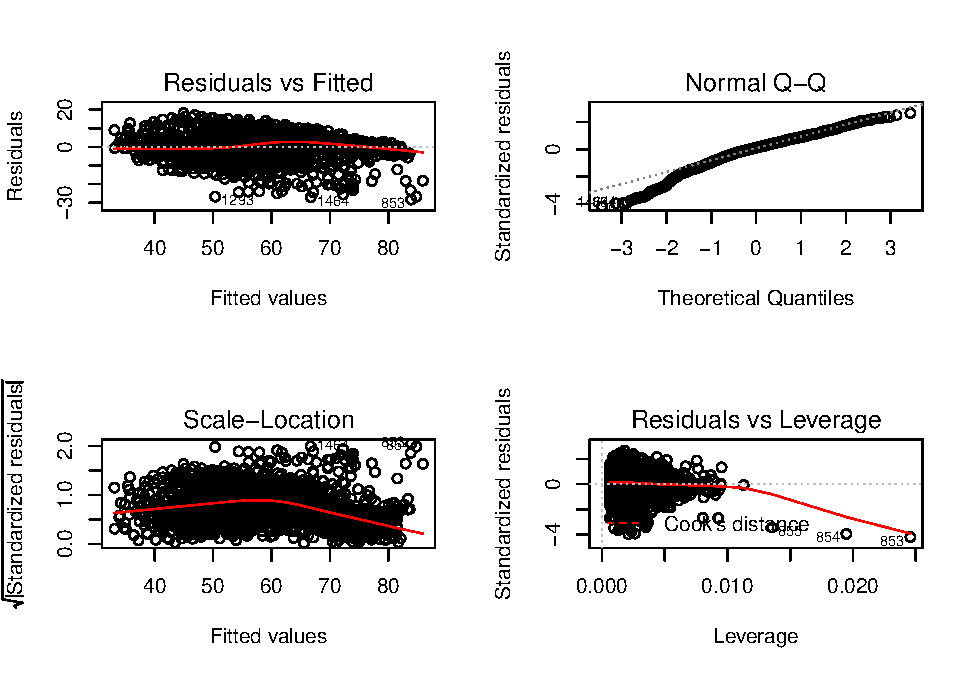
\includegraphics{08-new-SEM_files/figure-latex/unnamed-chunk-5-1.pdf} La
matrice de corrélation montre des corrélations élevées entre la plupart
de nos variables, mais elle ne nous dit rien sur les relations entre
elles. Un modèle théorique basé sur la littérature est proposé pour
expliquer les liens entre nos variables et le processus sous-jacent de
la croissance:

\begin{figure}
\centering
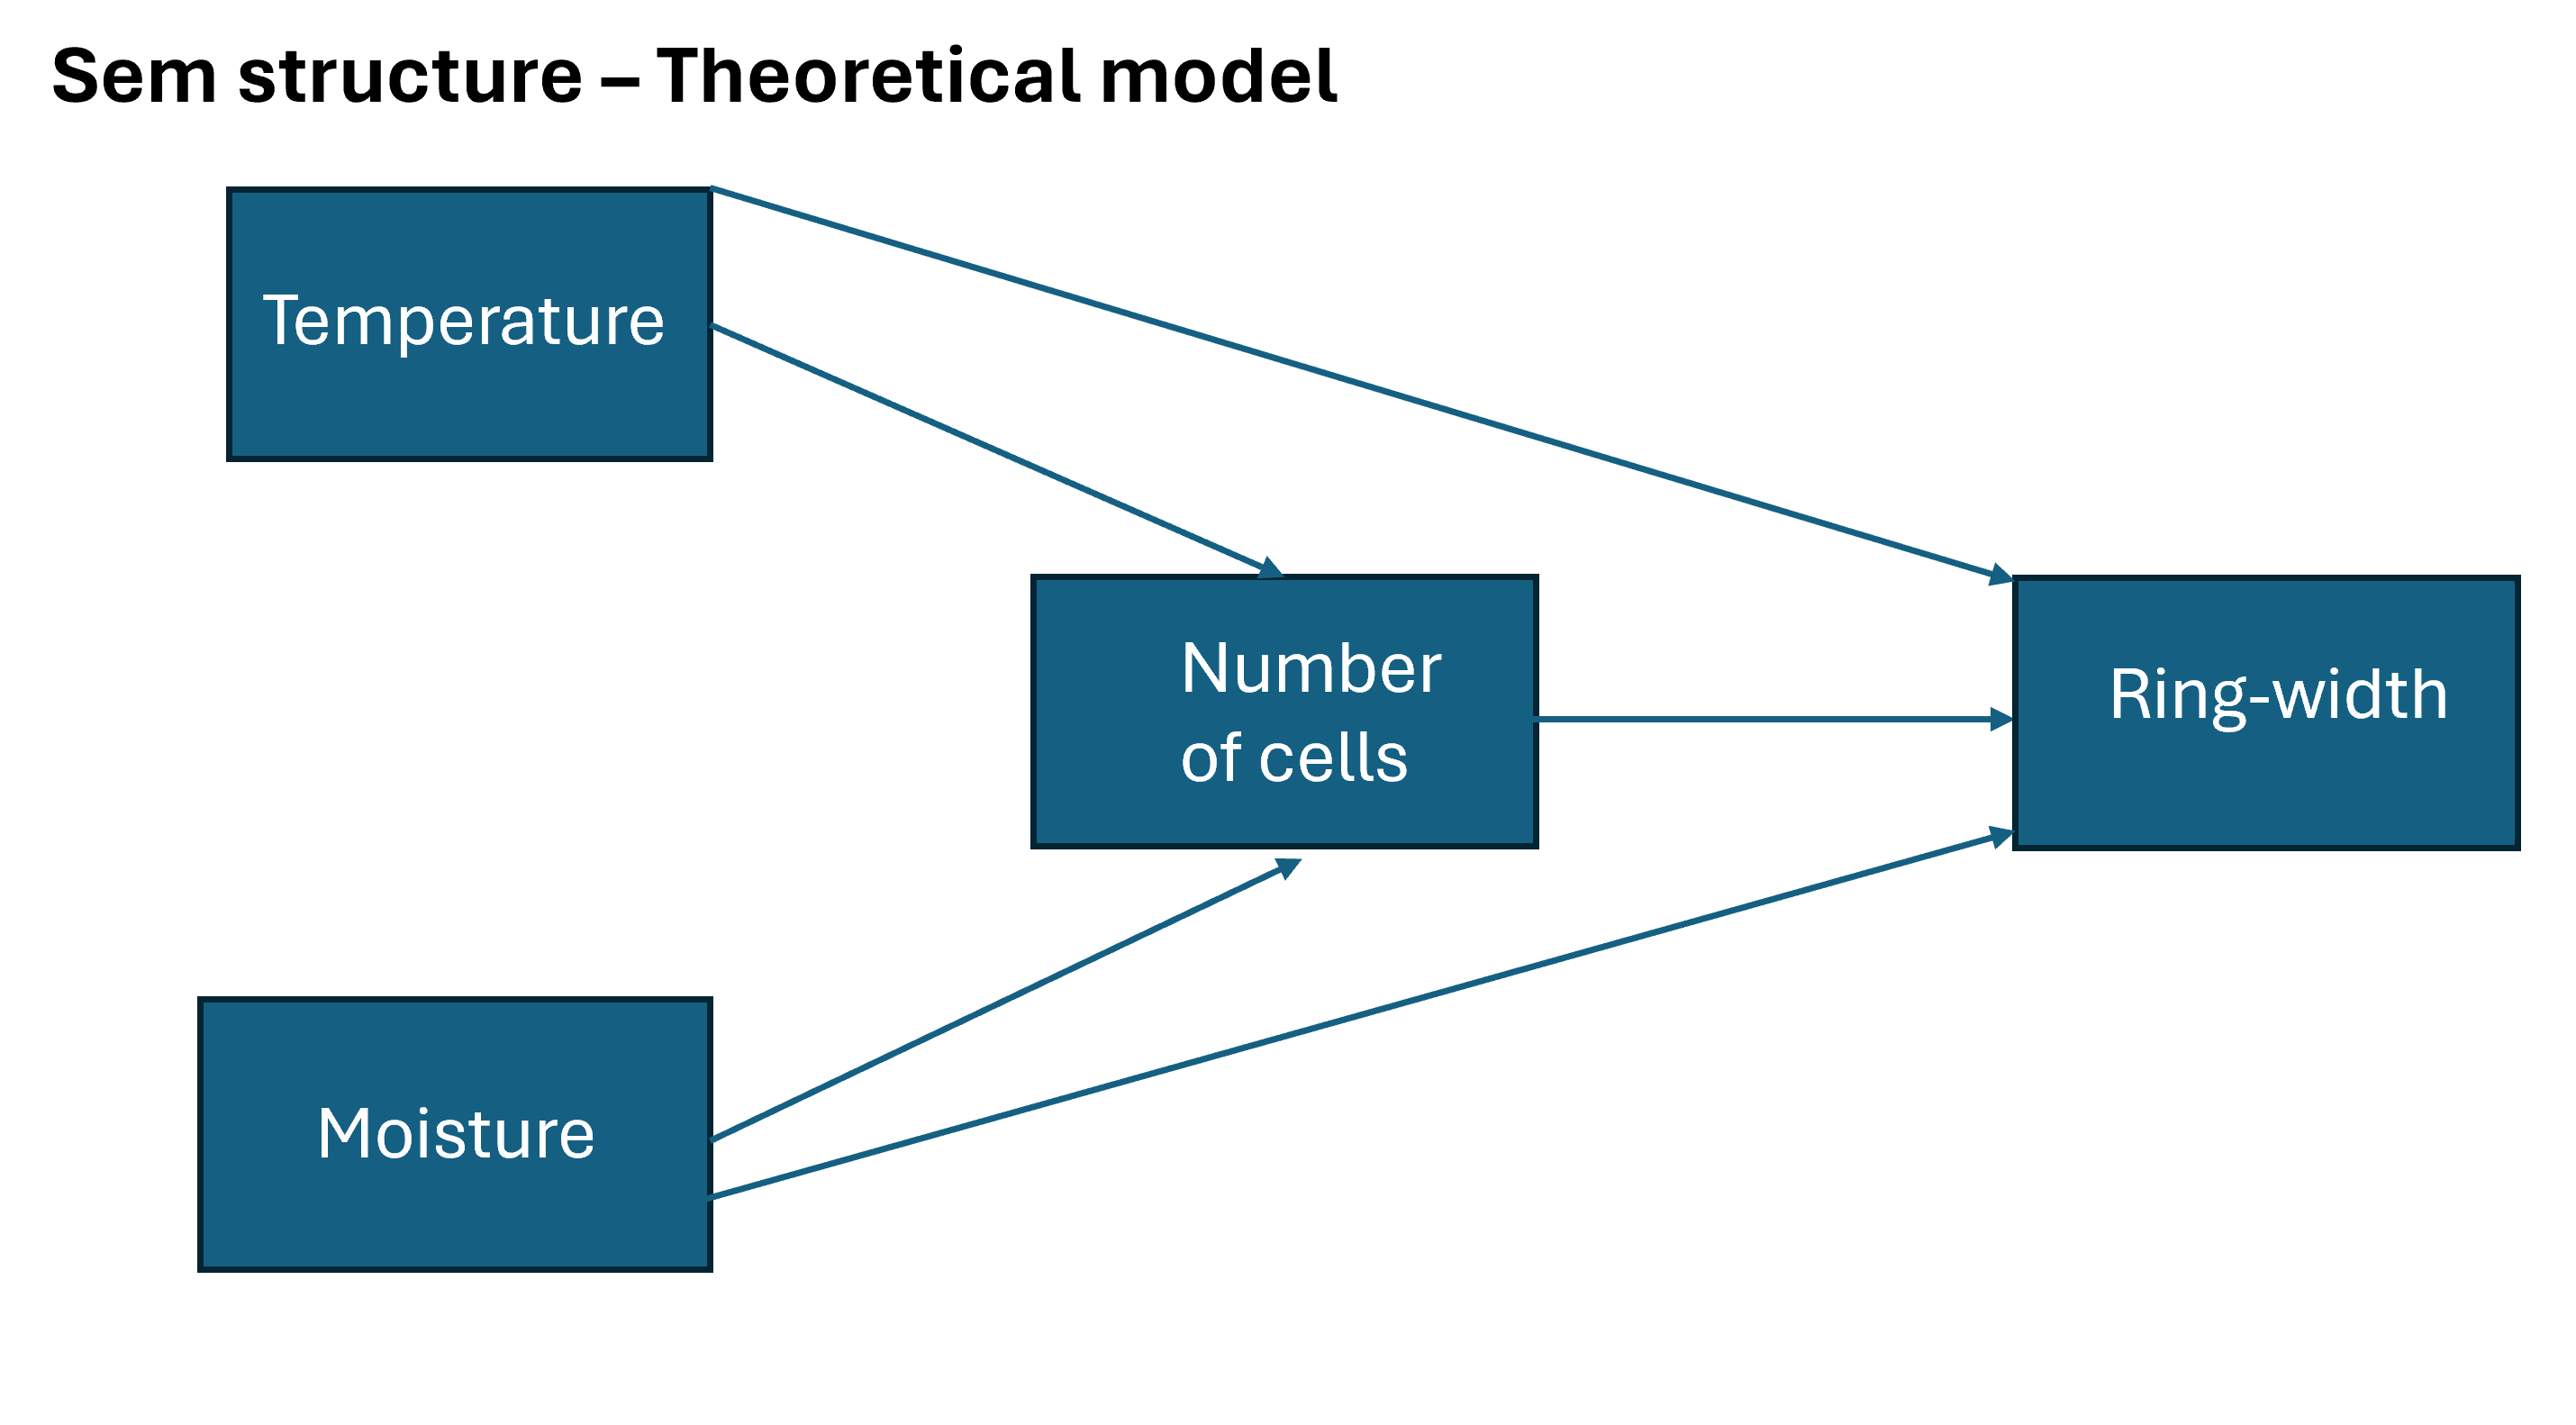
\includegraphics{C:/Users/buttoval/Documents/ECL8202/notes_cours/sem_exemple_2.png}
\caption{Relations entre les facteurs environnementaux et la croissance:
chaque lien est appuyé par des source de litterature}
\end{figure}

Sur lavaan, nous pouvons traduire le modèle avec la syntax suivante:

\begin{Shaded}
\begin{Highlighting}[]
\FunctionTok{require}\NormalTok{(lavaan)}
\end{Highlighting}
\end{Shaded}

\begin{verbatim}
## Le chargement a nécessité le package : lavaan
\end{verbatim}

\begin{verbatim}
## This is lavaan 0.6-15
## lavaan is FREE software! Please report any bugs.
\end{verbatim}

\begin{verbatim}
## 
## Attachement du package : 'lavaan'
\end{verbatim}

\begin{verbatim}
## L'objet suivant est masqué depuis 'package:psych':
## 
##     cor2cov
\end{verbatim}

\begin{Shaded}
\begin{Highlighting}[]
\NormalTok{myModel }\OtherTok{\textless{}{-}} \StringTok{\textquotesingle{} }

\StringTok{ \# regressions}
\StringTok{   ring\_width \textasciitilde{} temperature + humidity+ cell\_number}
\StringTok{   cell\_number \textasciitilde{}  temperature + humidity }
\StringTok{   cell\_number \textasciitilde{} \textasciitilde{}  stem\_size }

\StringTok{\textquotesingle{}}

\NormalTok{fit }\OtherTok{\textless{}{-}} \FunctionTok{sem}\NormalTok{(}\AttributeTok{model =}\NormalTok{ myModel, }
           \AttributeTok{data =}\NormalTok{ simulated\_data)}

\FunctionTok{summary}\NormalTok{(fit)}
\end{Highlighting}
\end{Shaded}

\begin{verbatim}
## lavaan 0.6.15 ended normally after 28 iterations
## 
##   Estimator                                         ML
##   Optimization method                           NLMINB
##   Number of model parameters                         9
## 
##   Number of observations                           200
## 
## Model Test User Model:
##                                                       
##   Test statistic                                 1.368
##   Degrees of freedom                                 3
##   P-value (Chi-square)                           0.713
## 
## Parameter Estimates:
## 
##   Standard errors                             Standard
##   Information                                 Expected
##   Information saturated (h1) model          Structured
## 
## Regressions:
##                    Estimate  Std.Err  z-value  P(>|z|)
##   ring_width ~                                        
##     temperature       0.343    0.187    1.832    0.067
##     humidity          0.235    0.105    2.239    0.025
##     cell_number       0.735    0.069   10.592    0.000
##   cell_number ~                                       
##     temperature       0.803    0.177    4.529    0.000
##     humidity          0.724    0.091    7.934    0.000
## 
## Covariances:
##                    Estimate  Std.Err  z-value  P(>|z|)
##  .cell_number ~~                                      
##     stem_size        30.682    9.433    3.253    0.001
## 
## Variances:
##                    Estimate  Std.Err  z-value  P(>|z|)
##    .ring_width      150.351   15.035   10.000    0.000
##    .cell_number     156.311   15.631   10.000    0.000
##     stem_size       107.827   10.783   10.000    0.000
\end{verbatim}

Le résumé de la fonction sem nous fournit ainsi les coefficients de
régression qui indiquent la force et la direction de la relation entre
nos variables. Les coefficients de covariance mesurent également la
force et la direction de la corrélation entre les variables. On peut
interpréter ces coefficients comme n'importe quels coefficients d'une
régression linéaire. Cependant, il peut être très utile de standardiser
la valeur des coefficients si l'on souhaite comparer l'effet des
différentes variables sur notre variable réponse.

\hypertarget{ajustement-du-moduxe8le-sur-lavaan}{%
\section{Ajustement du modèle sur
Lavaan}\label{ajustement-du-moduxe8le-sur-lavaan}}

On considère qu'un SEM représente bien notre distribution de données et
notre phénomène naturel lorsque le p-value (chi carré) du modèle n'est
pas significatif. Cela arrive parce que nous souhaitons observer une
correspondance entre les données observées et les prédictions de notre
modèle, lesquelles ne doivent pas présenter de différences
significatives. Dans ce cas, le p-value est de 0.713, ce qui nous
rassure quant à la capacité du modèle à représenter notre phénomène.Il
est également utile de vérifier d'autres mesures d'ajustement du modèle,
pour obtenir une évaluation plus complète de l'adéquation du modèle.
Voici les indicateurs plus courentment utilisés. Voici une synthèse
présentée par Joreskog, K., \& Sorbom, D. (1993):

\begin{figure}
\centering
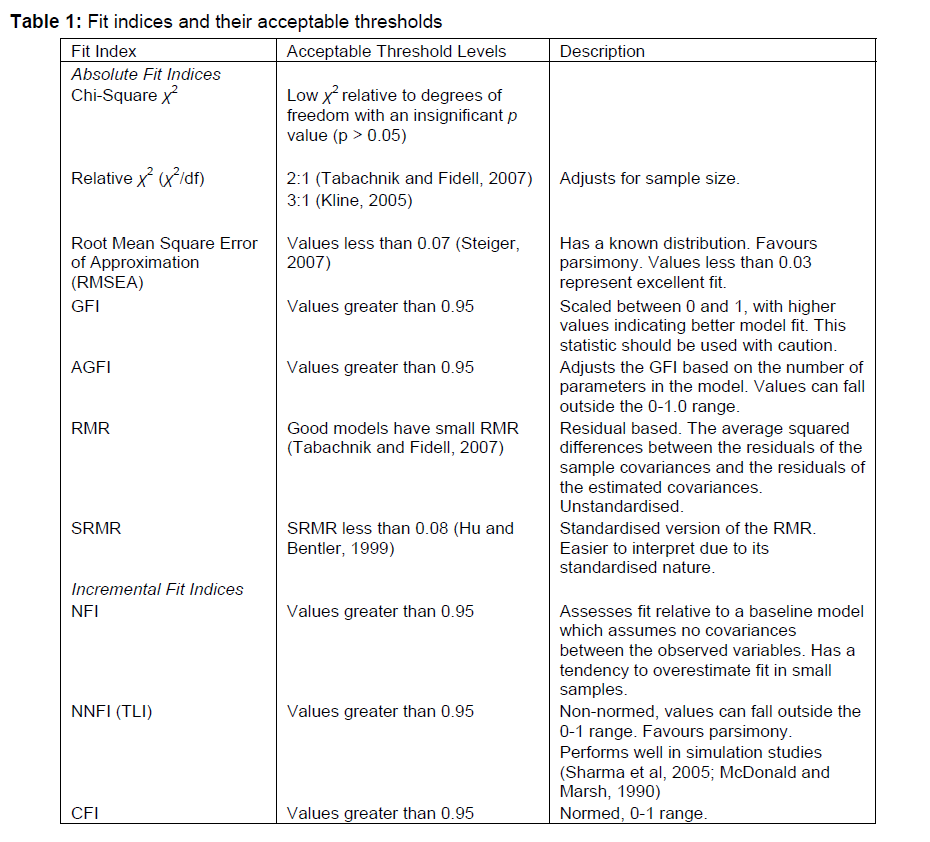
\includegraphics{C:/Users/buttoval/Documents/ECL8202/notes_cours/table1_index.PNG}
\caption{Ajoustement du modèle}
\end{figure}

il est possible de trouver ces metriques d'ajoustement pour notre modèle
grace à la fonction: fitMeasures()

\begin{Shaded}
\begin{Highlighting}[]
\FunctionTok{fitMeasures}\NormalTok{(fit, }\FunctionTok{c}\NormalTok{(}\StringTok{"chisq"}\NormalTok{, }\StringTok{"df"}\NormalTok{, }\StringTok{"pvalue"}\NormalTok{, }\StringTok{"cfi"}\NormalTok{, }\StringTok{"rmsea"}\NormalTok{))}
\end{Highlighting}
\end{Shaded}

\begin{verbatim}
##  chisq     df pvalue    cfi  rmsea 
##  1.368  3.000  0.713  1.000  0.000
\end{verbatim}

Il existe des standards pour nous naviguer dans la présentation de ces
indicateurs:

\begin{figure}
\centering
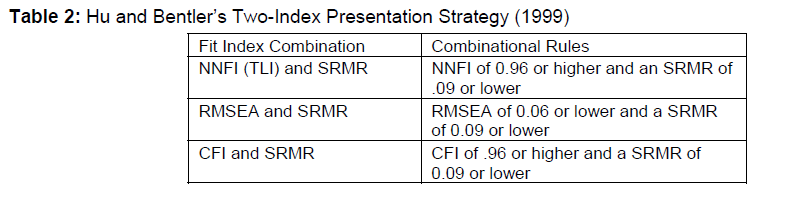
\includegraphics{C:/Users/buttoval/Documents/ECL8202/notes_cours/table2_index.PNG}
\caption{Combinaisons d'indicateurs d'ajoustement}
\end{figure}

\begin{Shaded}
\begin{Highlighting}[]
\FunctionTok{summary}\NormalTok{(fit,}\AttributeTok{standardized=}\ConstantTok{TRUE}\NormalTok{)}
\end{Highlighting}
\end{Shaded}

\begin{verbatim}
## lavaan 0.6.15 ended normally after 28 iterations
## 
##   Estimator                                         ML
##   Optimization method                           NLMINB
##   Number of model parameters                         9
## 
##   Number of observations                           200
## 
## Model Test User Model:
##                                                       
##   Test statistic                                 1.368
##   Degrees of freedom                                 3
##   P-value (Chi-square)                           0.713
## 
## Parameter Estimates:
## 
##   Standard errors                             Standard
##   Information                                 Expected
##   Information saturated (h1) model          Structured
## 
## Regressions:
##                    Estimate  Std.Err  z-value  P(>|z|)   Std.lv  Std.all
##   ring_width ~                                                          
##     temperature       0.343    0.187    1.832    0.067    0.343    0.096
##     humidity          0.235    0.105    2.239    0.025    0.235    0.128
##     cell_number       0.735    0.069   10.592    0.000    0.735    0.618
##   cell_number ~                                                         
##     temperature       0.803    0.177    4.529    0.000    0.803    0.267
##     humidity          0.724    0.091    7.934    0.000    0.724    0.467
## 
## Covariances:
##                    Estimate  Std.Err  z-value  P(>|z|)   Std.lv  Std.all
##  .cell_number ~~                                                        
##     stem_size        30.682    9.433    3.253    0.001   30.682    0.236
## 
## Variances:
##                    Estimate  Std.Err  z-value  P(>|z|)   Std.lv  Std.all
##    .ring_width      150.351   15.035   10.000    0.000  150.351    0.497
##    .cell_number     156.311   15.631   10.000    0.000  156.311    0.730
##     stem_size       107.827   10.783   10.000    0.000  107.827    1.000
\end{verbatim}

\hypertarget{ruxe9ferences}{%
\subsection{Réferences}\label{ruxe9ferences}}

Revelle, 2024: How to use the psych package for regression and mediation
analysis:
\url{https://cran.r-project.org/web/packages/psychTools/vignettes/mediation.pdf}

Yves Rosseel (2012). lavaan: An R Package for Structural Equation
Modeling. Journal of Statistical Software, 48(2), 1-36. URL
\url{http://www.jstatsoft.org/v48/i02/} \url{https://lavaan.ugent.be/}

Joreskog, K., \& Sorbom, D. (1993). Structural equation modelling:
Guidelines for determining model fit. NY: University Press of America.

\end{document}
